\documentclass[11pt]{article}
\usepackage{amsmath}
%\usepackage{extsizes}
\usepackage{amsmath,amssymb}
%\usepackage{omegavn,ocmrvn}
%\usepackage[utf8x]{inputenc}
\usepackage[utf8]{vietnam}

\usepackage{longtable}
\usepackage{answers}

\usepackage{graphicx}
\usepackage{float}

\usepackage{array}
\usepackage{pifont}
\usepackage{picinpar}
\usepackage{enumerate}
\usepackage[top=3.0cm, bottom=3.5cm, left=3.5cm, right=2.5cm] {geometry}
\usepackage{hyperref}


\newtheorem{bt}{Câu}
\newcommand{\RR}{\mathbb R}
\Newassociation{sol}{Solution}{ans}
\newtheorem{ex}{Câu}
\renewcommand{\solutionstyle}[1]{\textbf{ #1}.}
\newcommand{\m}[1]{\begin{bmatrix}
		#1
\end{bmatrix}}

\begin{document}
% \noindent
\begin{tabular*}
{\linewidth}{c>{\centering\hspace{0pt}} p{.7\textwidth}}
Trường ĐHKHTN, ĐHQGHN & {\bf Học Kỳ 1 (2018-2019)}
\tabularnewline
K61 TTƯD & {\bf Bài Tập Giải Tích Số. No 11 \\ Giải hệ pt tuyến tính Ax=b}
% Exercises on pages 239, 240 Cheney/Kincaid are really nice
\tabularnewline
\rule{1in}{1pt}  \small  & \rule{2in}{1pt} %(Due date:)
\tabularnewline

%  \tabularnewline
%  &(Đề thi có 1 trang)
\end{tabular*}
%
% \Opensolutionfile{ans}[ans1]
\vskip .2cm

Đối với 2 bài tập đầu, hãy viết hàm trong MATLAB dạng $x=low\_sys(L,z)$ (hoặc $x=upp\_sys(R,z)$) để giải hệ phương trình $Lx = z$ (t.ứ. $Rx = z$) với $L$ (t.ứ. $R$) là ma trận tam giác dưới (t.ứ. tam giác trên).

\begin{bt}
Để giải hệ phương trình $Ax=b$ với $A\in \mathbb{R}^{n,n}$, $n\leq 10^5$, các phương pháp Gauss và phần tử trội thường được dùng. Hãy giải hệ phương trình sau bằng các phương pháp đó (sử dụng các phân tích $lu$ tương ứng trong MATLAB).
%
\begin{align*}
 2 x_1 + 4 x_2 + 3x_3   &= 3, \\
 3 x_1 + x_2 - 2 x_3    &= 3, \\
 4 x_1 + 11 x_2 + 7 x_3 &= 4. 
\end{align*}
%
Chú ý tìm hiểu các lệnh $[L,U]=lu(A)$, và $[L,U,P]=lu(A)$. So sánh kết quả với việc dùng lệnh $x=A \backslash b$.
\end{bt}

\begin{bt} Giả sử ma trận $A$ thỏa mãn $PA = LU$, trong đó
\begin{figure}[h!]
	\centering
	
\includegraphics[scale = 0.7]{3}
\end{figure}
a) Hãy sử dụng các ma trận trên để giải hệ phương trình $Ax=b$ với $b = \m{2 & 10 & -12}^T$ mà không cần tìm ma trận $A$ hay tìm nghich đảo của $A$.
b, Có thể nhận thấy ma trận P nhận được từ ma trận đơn vị bằng cách hoán vị các hàng. Hãy nêu ý nghĩa của việc nhân một ma trận với $P$ từ bên trái.
\end{bt}

\begin{bt}
	Trong trường hợp ma trận A là đối xứng, xác định dương thì phương pháp Cholesky thường được sử dụng. Hãy đọc phương pháp này trang 177-178 (Giáo trình) và tìm hiểu lệnh $R = chol(A)$ trong MATLAB. Áp dụng để giải hệ phương trình sau đối với vế phải $b$ lần lượt bằng $[2 \ 3 \ 0]^T$ và $[2 \ 5 \ -2]^T$.
	%
	\begin{align*}
	4 x_1 - 2 x_2 + 4 x_3   &= b_1, \\
	-2 x_1 + 5 x_2 - 4 x_3  &= b_2, \\
	4 x_1  -4 x_2 + 6 x_3   &= b_3. 
	\end{align*}
	%
\end{bt}

\begin{bt} 
Để xác định số điều kiện $\kappa(A) = \|A\| \cdot \|A^{-1}\|$ của ma trận $A$, ta cần đi tính chuẩn của ma trận đó. Hãy tìm chuẩn và số điều kiện tương ứng của $A=\m{4 & 1 \\ 2 & 2}$ trong các trường hợp  $\|\cdot\|_{1}$ và $\|\cdot\|_{\infty}$. So sánh kết quả tìm được với kết quả khi dùng lệnh $norm(A,1)$ và $norm(A,inf)$ trong MATLAB.
\end{bt}

\newpage 

\begin{bt}
\end{bt}

\begin{center}
  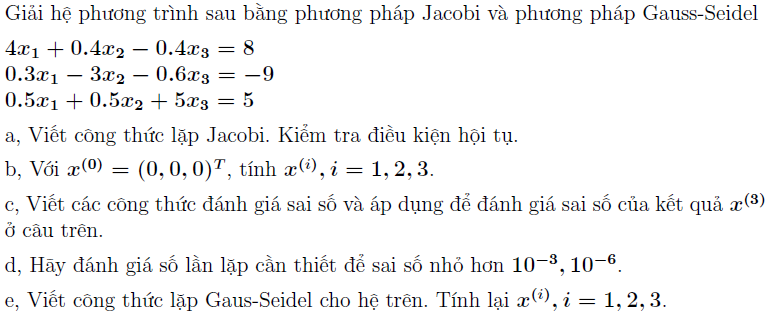
\includegraphics[scale = 0.7]{4}	
\end{center}

\begin{bt}
\end{bt}
\begin{figure}[H]
	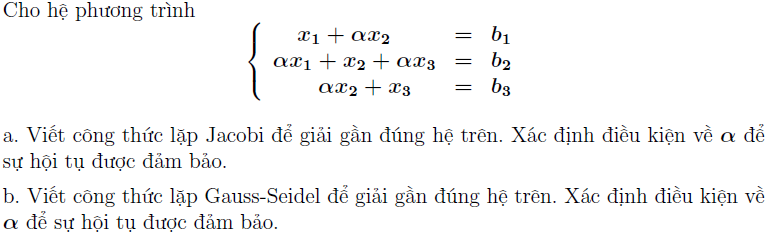
\includegraphics[scale = 0.7]{5}
\end{figure}
c. Từ các tính toán ở hai câu trên, hãy so sánh tốc độ hội tụ của hai phương pháp.

\vskip .5cm

\centerline{———————————Hết——————————-}

\end{document}

\vspace{1cm}
\noindent{\bf Chú ý:} {\it Cán bộ coi thi không giải thích gì thêm}\\
\Closesolutionfile{ans}
\newpage
\begin{center}
{\LARGE{\bf ĐÁP ÁN}}
\end{center}

\begin{sol}
	\begin{figure}[h!]
		\centering
		\includegraphics[width=0.8\linewidth]{Solution1/Sol4_1.png}
		%\caption{}
		\label{fig:Sol4}
	\end{figure}
	Exercise 7: Convergence order is 3.	
\end{sol}

   
\end{document}



